%\documentclass{article}
%\usepackage{graphicx}
%\newcommand{\bc}{\begin{center}}
%\newcommand{\ec}{\end{center}}
%\newcommand{\be}{\begin{equation}}
%\newcommand{\ee}{\end{equation}}
%\newcommand{\bea}[1]{\begin{eqnarray}\label{#1}}
%\newcommand{\eea}{\end{eqnarray}}
%\newcommand{\bua}{\begin{eqnarray*}}
%\newcommand{\eua}{\end{eqnarray*}}
%\newcommand{\dd}[2]{{{d#1}\over{d#2}}}
%\newcommand{\ddt}[1]{\dd{#1}{t}}
%\newcommand{\dddt}[1]{\dd{^2#1}{t^2}}
%\newcommand{\aver}[1]{\langle{#1}\rangle}
%\begin{document}
\chapter{The human eye}
% Maybe remove the whole chapter from the course?
The human eye is not much in use as a professional tool of
astronomy. On the other hand, it is of great interest to understand how it
works and by doing so we may illustrate many of the principles and
problems that we will meet later in the course.

Evolution has come up with different designs for eyes, but most (if
not all) can be divided into two parts\footnote{Some of the
  information here is gathered from the highly recommended book by
  Nick Lane {\it Life Ascending, the ten great inventions of
    evolution}, Richard Dawkins' {\it Climbing Mount
    Improbable} also contains a chapter on the evolution of the eye.}:
{\it a lens}, or set of lenses, for
focussing light onto a {\it receptor} which detects light and sends
information of detection on to the brain or nervous system. There are
many designs and materials used for the optical set up of the
lens. For example trilobites, perhaps the first animals to develop
eyes some 540~million years ago during the Cambrian, used lenses made
of crystal, the mineral calcite. Calcite has many interesting optical
properties, amongst which is the fact that they deflect light from all
angles, except one privileged axis called the {\it c}-axis. Each eye
facet in a trilobite had its own calcite lens directed so that light
would pass in only one direction to the underlying retina. While there
are many designs for lenses, all light detecting cells see to be based
on a single protein, or molecule, called {\it rhodopsin}, perhaps
pointing to a common evolutionary source for all eyes extant
throughout the animal kingdom\footnote{Note that the design
  of light sensitive cells is roughly divided into two groups, where
  all the vertebrates share a similar design and the invertebrates another.}.

The eye and brain work together, and the brain can correct for many of
the aberrations suffered by the eye. Thus, for example, the brain compensates for
the fact that the image on the retina is inverted, and for chromatic
aberration. 

\begin{figure}[h!]
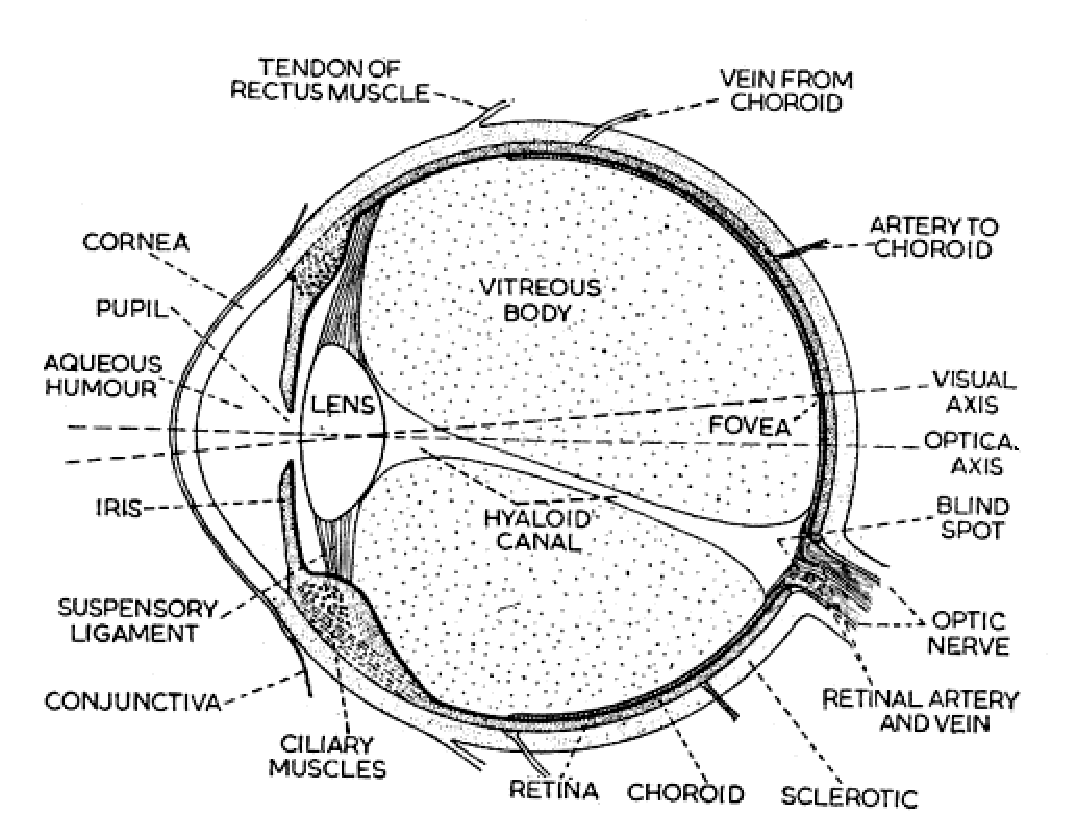
\includegraphics[width=0.49\textwidth]{eye-schematic.eps}
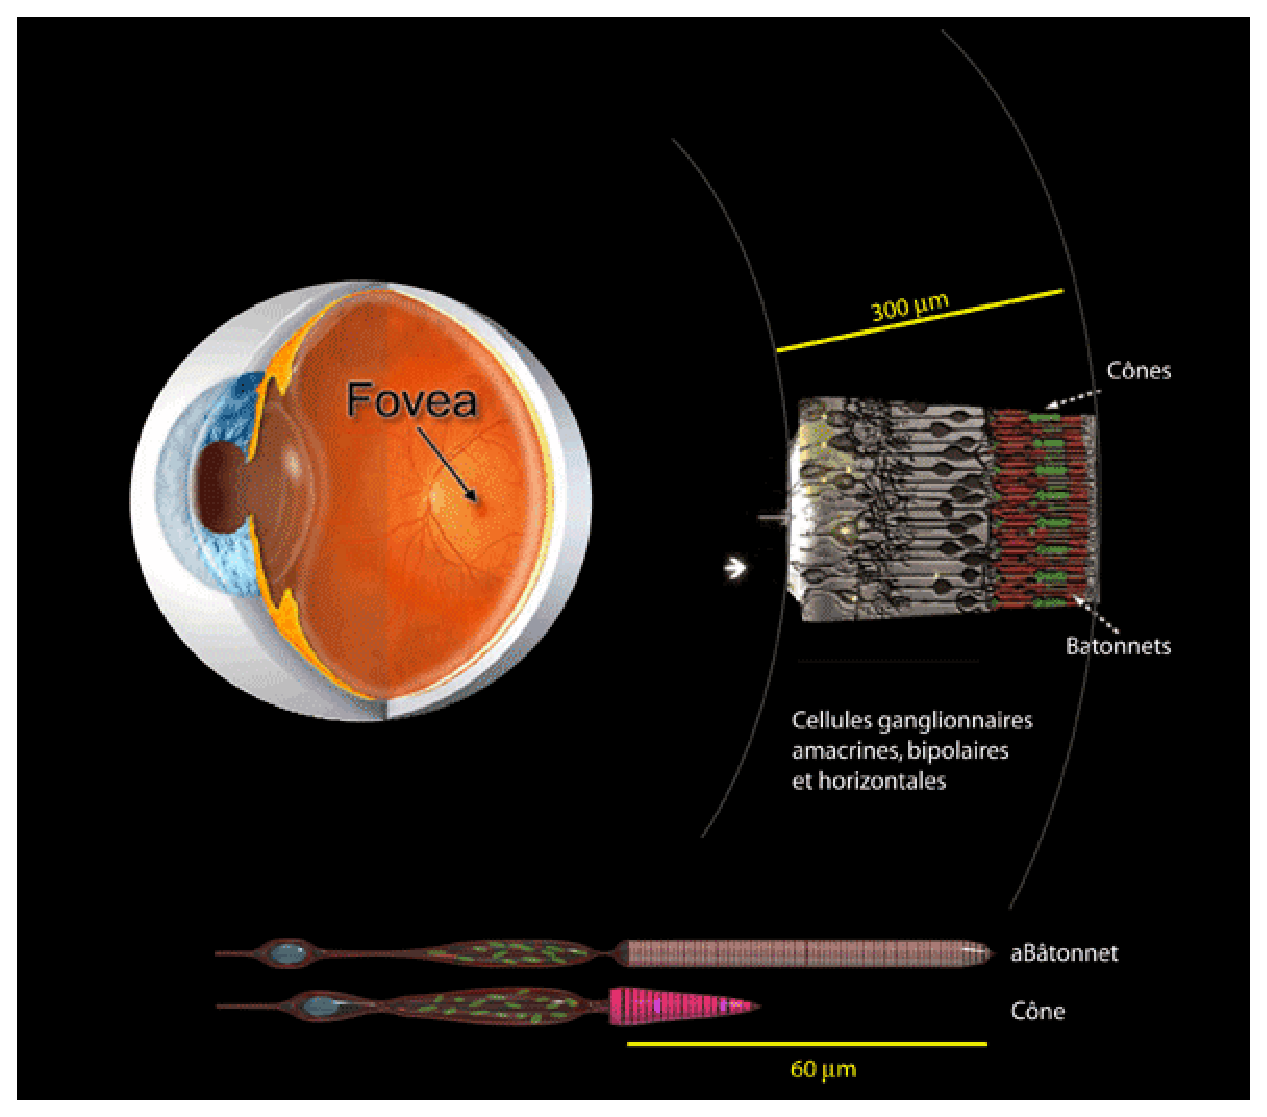
\includegraphics[width=0.49\textwidth]{eye-rod-cone.eps}
\caption{Cross section of the human eye (left), illustration of the eyes
receptor cells; cones, used for color vision with the iodopsin layers 
arranged to the right, and rods with rhodopsin layers. Light enters these
cells from the left before being absorbed by either iodopsin or rhodopsin.}
\end{figure}

Light is focussed on the retina, where there are two types of
receptors: rods and cones. Cones for color reception, rods for black
and white with higher sensitivity. For humans, rods and cones are
arranged {\it backwards} so light must pass through the neuronal wires
that send signals of light back to the brain. In contrast, octopus
eyes, which otherwise are much as our own with a single lens in front
and a light sensitive retina at the back, has the light sensitive
parts of the retinal cells in front. This may be an accident of
nature, or there may be good evolutionary reasons for
the difference. Both designs are mimicked in CCD's used in astronomy,
where {\it thinned, backlit} CCDs are used to avoid unwanted reflections from
the electrodes used to drive them. The CCD in your camera or cell
phone is more probably arranged in the same manner as your eye, with
light having to pass through the electrodes lying on top of light
sensitive doped silicon.

In the rods a pigment known as rhodopsin absorbs radiation. A protein
with a weight of some $40\,000$~amu, arranged in layers 20~nm thick
and 500~nm wide. Under influence of light a small fragment, a
chromophore, will will split off. The chromophore is a vitamin A
derivative called retinal (or retinaldehyde) with a molecular weight
of 286~amu. The portion left behind is a colorless protein called opsin. 
The moment of visual excitation occurs during this break
off process as the cell's electrical potential increases (for
invertebrates on the other hand excitation occurs because the
electrical charge across the membrane is removed). This change in
potential can then propagate along nerve cells to the brain. The
rhodopsin molecule is then (slowly) regenerated. 

The response of cones is similar, but in this case the pigment is
known as iodopsin which also contains the retinaldehyde group. Cone
cells come in three varieties with different spectral sensitivities
(see figure~\ref{fig:absorption-rod-cone}).

In bright light much of the rhodopsin is broken up into opsin and
retinaldehyde, and the rod sensitivity is much reduced so that vision
is primarily provided by the cones, even though their light sensitivity
is only of order 1\% of the rods. The three varieties of cones combine
to give color vision. At low light levels only rods are triggered by
the ambient radiation and vision is then in black and white. 

\begin{figure}[h!]
\centering
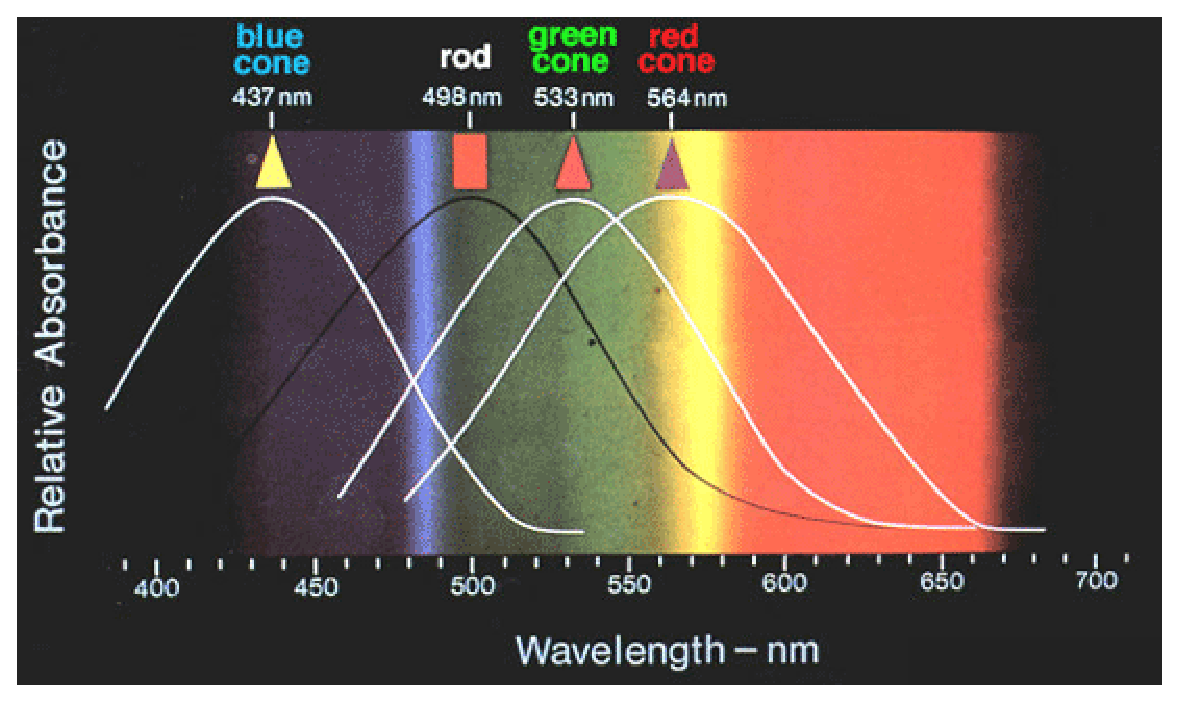
\includegraphics[width=0.66\textwidth]{absorption-rod-cone.eps}
\caption{Absorption curves for the various types of cones, which combined
give color vision, and for rhodopsin. Note that the peak sensitivity
for rods (at 500~nm) and cones (at 555~nm) are at different wavelengths: this causes the
sensitivity of the eye to shift towards blue at low light levels when
the rods dominate.}
\label{fig:absorption-rod-cone}
\end{figure}

Upon entering the dark from a brightly lit region rhodopsin will build
up over a period of roughly 30~min, thus dark-adaptation takes this
long and is based on rod cells. Somewhere between 1--10 photons are
necessary to trigger an individual rod. However, several rods must be
triggered in order to result in a pulse being sent to the brain, as
many rods can be connected to a single nerve fibre. The total number
of rods is of order $10^8$, of cones $6\times 10^6$, these must share
some $10^6$ nerve fibres. Thus there are roughly 100 visual receptors
per nerve fibre, note that there can be many cross connections between
groups of receptors. Cones are concentrated towards the fovea
centralis, which is the region of most acute vision, while rods are
most plentiful towards the periphery of the field of view. Weak
objects are thus most easily visible with averted vision, {\it ie}
when it is not looked at directly. In sum with all these effects the
eye is usable over a range of illuminations differing by a factor
$10^9$ -- $10^{10}$. Note that in regions of high contrast the
brighter region is often seen as too large, this is a phenomena known
as {\it irradiation}. It arises from stimulated responses of unexcited
receptors due to their cross connection with excited receptors. Eye
fatigue occurs when staring fixedly at a source for an extended period
due to depletion of the sensitive pigment.

The Rayleigh limit of the eye, roughly given by $\lambda/D$ where
$\lambda$ is the wavelength of the observed light and $D$ is the size
of the observing aperture, is of order 20~arcsec when the iris has
its maximum diameter of 5--7~mm. However, for two separate images to
be distinguished, they must be separated by at least one unexcited 
receptor cell, so even on the fovea centralis resolution is limited in
practice to between 1~arcmin and 2~arcmin. This is much better than
elsewhere on the retina, since the fovea centralis is populated by
small, tightly packed, singly connected cones. The average resolution
of the eye lies between 5~arcmin and 10~arcmin for point sources. Linear
sources such as an illuminated grating can be resolved down to 1~arcmin.  
The effect of granularity of the retina is countered by rapid oscillations of the
eye through a few 10~arcsec with a frequency of a few Hz, so that
several receptors are involved in the detection when averaged over
time.

The response of the eye to changes in illumination is logarithmic; if
two sources $A$ and $B$ are observed to differ by a given amount, and a
third source $C$ is seen to lie midway between them, then the energy
from $C$ will differ from $A$ by the same factor as it differs from
$B$. The faintest stars visible at a good site (magnitude $6^{\rm m}$)
corresponds to a detection of approximately $3\times
10^{-15}$~W. Sensitivity will vary between individuals and decreases
with age, the retina of a 60~year old person will receive some 30\% of 
the light seen by a person of 30-years.

The system used by astronomers to measure the brightness of stars is a
very old one, and is based on the sensitivity of the eye. Hipparchos'
catalogue of stars divided the stars into six classes from the
brightest, of the first rank or magnitude, to the dimmest of the sixth
magnitude. The present day system is based on this after the work of
Norman Pogson put the magnitude scale on a firm basis in 1856. Pogson
suggested a logarithmic scale that approximately agreed with earlier
measurements: the difference between stars of magnitude $m_1$ and
$m_2$ are given by 
\[
m_1-m_2=-2.5\log\left({E_1\over E_2}\right)
\]
where $E_1$ and $E_2$ are the energies per unit area at the surface of
Earth for the two stars.

\section{Exercises}

\begin{enumerate}
\item What is the size, in kilometers, of the smallest crater that can be distinguished on 
the Moon with the naked eye (as seen from Earth)?
\item Vega has a magnitude of roughly $0.0$, Polaris a magnitude of $2.0$. 
Estimate the magnitudes of the stars in Orions belt as well as Betelgeuse,
Rigel, and Bellatrix. What is the magnitude of the weakest star you can find
in the sky? 
\item Mizar and Alcor in Ursa Majoris are separated by some $11'$.
 Can you separate them and see both stars? Estimate their magnitudes
 as well. Mizar is itself a double star the components of which can be
 separated with a small telescope. Interestingly, all three stars are
 {\it spectroscopic binaries} as well, bringing the star total star
 count up to 6. The distance to these stars is some 83~ly while the
 distance between Mizar and Alcor is approximately
 1~ly. All six stars are  gravitationally bound and are
 members of the Ursa Major moving group.
\end{enumerate}

%\end{document}
